The second stage of offline training was to go further than just mimicking expert human moves. Silver et al.\cite{b12} wanted AlphaGo to learn new, improved policies on its own. Policy gradient RL techniques were applied to the SL policy network to get an improved reinforcement learning (RL) policy network, $p_\rho$ (identical in structure to SL policy network). In RL literature, they are termed ubiquitously as \textit{behavior policy} and \textit{target policy}. The new, improved policy being learned is called the target policy (in our case, RL policy), and the policy used to generate behavior is called the behavior policy (in our case, SL policy). The weights of the RL policy network were first initialized as $\rho = \sigma$. Next, games were played using the new RL policy network against randomly selected from the set of older RL policy networks. Games were not played with the same policy network to avoid overfitting the current policy (i.e., it will memorize the moves rather than generalize them for different opponents). The game is played till the terminal state. A reward function $r(s)$ that is zero for all non-terminal time steps $t<T$ was used. The outcome $z_t = \pm r(s_T)$ is the terminal reward at the end of the game from the perspective of the current player at time step t: $+1$ for winning and $-1$ for losing. The weights of the RL policy network are updated similarly to the SL policy network, except we use the game result $z_t$ to determine which direction to move in the stochastic gradient ascent that maximizes this expected outcome $z_t$,
\begin{equation}
    \nabla \rho \propto \frac{\partial \log p_\rho (a_t|s_t)}{\partial \rho}z_t.
\end{equation}

\begin{figure}[b]
\centerline{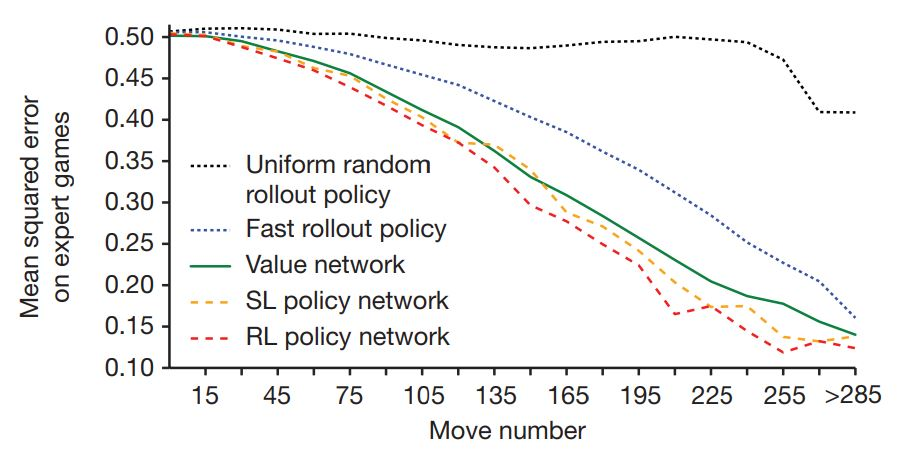
\includegraphics[width = 0.8\columnwidth]{RL_acc.JPG}}
\caption{Accuracy of reinforcement learning value network\cite{b12}}
\label{RL_accu}
\end{figure}